\chapter{Aufbau des Verfahrens}

Um nun aufbauend auf diesen Erkenntnissen die allgemeinen Flugbahnen beliebiger Ladungstr\"ager durch beliebige, unter Umst\"anden
auch \textit{inhomogene}, Magnetfelder simulieren zu k\"onnen, sind mehrere Zwischenschritte notwendig.
Unter Verwendung der Ergebnisse aus dem vorigen Abschnitt wird zun\"achst ein Verfahren hergeleitet, welches es erm\"oglicht,
die Teilchenflugbahnen in \textit{homogenen} Magnetfeldern zu simulieren. Dieses Verfahren kann anschlie{\ss}end auf beliebige
Magnetfelder ausgeweitet werden, indem man diese abschnittsweise durch homogene Teilfelder approximiert, auf welchen dann das
hergeleitete Verfahren zur Anwendung kommt.

\section{Simulation der Flugbahn im homogenen Magnetfeld}

Bewegen sich Teilchen im Raum, so kann dies in allen m\"oglichen Orientierungen erfolgen. Um diesem Sachverhalt Rechnung zu tragen,
werden zun\"achst s\"amtliche Schritte im lokalen Bezugssystem des Ladungstr\"agers durchgef\"uhrt. Unabh\"angig von der speziellen
Orientierung des Teilchens gew\"ahrleistet dies einheitliche Rechenvorschriften, welche im Anschluss durch einfache
Basistransformationen in das globale Koordinatensystem \"uberf\"uhrt werden k\"onnen. Die gr\"o{\ss}en \(v\) und \(B\), welche
im vorigen Abschnitt noch als Skalare betrachtet wurden, m\"ussen nun \textit{vektoriell} als \(\vec{v}\) und \(\vec{B}\)
aufgefasst werden. Es wird sich aber zeigen, dass dies durch die geeignete Wahl der lokalen Basisvektoren nur eine untergeordnete Rolle
spielt.

\subsection{Die Flugbahn im lokalen Bezugssystem des Ladungstr\"agers}
\label{sec:lokales_bezugssystem}

Das lokale Koordinatensystem wird nun so gew\"ahlt, dass sich die Position des Teilchens genau im Ursprung befindet.
Weiterhin zeigen die magnetischen
Feldlinien genau in Richtung der \textit{z-Achse}, die orthogonale Projektion der Teilchenbewegung auf die xy-Ebene zeigt genau
entlang der \textit{y-Achse}, wie in \fref{fig:locale_movement} dargelegt. Auf diese Weise lassen sich die beiden Anteile der
Bewegung optimal trennen: Der gleichf\"ormige Anteil, welcher auf \(v_\parallel\) zur\"uckzuf\"uhren ist,
verl\"auft genau entlang der \textit{z-Achse}, w\"ahrend \(v_\perp\) eine Kreisbewegung in der \textit{xy-Ebene} verursacht.
\(v_\parallel\) beeinflusst also nur die \textit{z-Koordinate} des Ladungstr\"agers, w\"ahrend \(v_\perp\) ausschlie{\ss}lich die
\textit{x}-, sowie die \textit{y-Koordinate} beeinflusst.

\begin{figure}
  \centering
  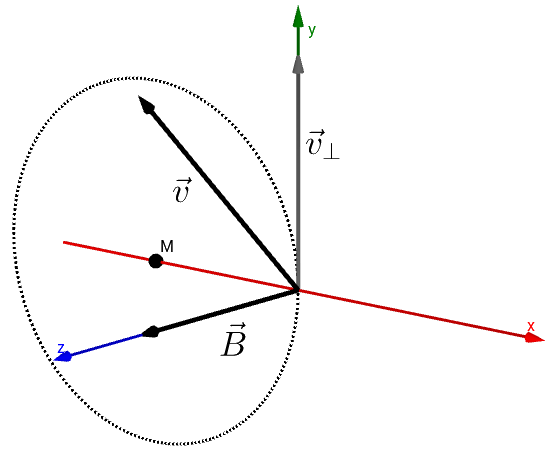
\includegraphics[width=0.6\textwidth]{geogebra/img/local_movement_edited}
  \caption{Das lokale Koordinatensystem des im Ursprung befindlichen Ladungstr\"agers mit Andeutung der Kreisbahn in der
    \textit{xy}-Ebene.}
  \label{fig:locale_movement}
\end{figure}

Um nun den Mittelpunkt \(M\) des Kreises zu ermitteln, welchem die Bewegung in der \textit{xy-Ebene} folgt, kann zun\"achst der
Radius \(r\) dieses Kreises bestimmt werden. Gem\"a{\ss} der Konstruktion und unter Ber\"ucksichtigung der \textit{Linke-Hand-Regel}
liegt \(M\) dann genau auf der \textit{x-Achse} und hat die xy-Koordinaten \(\left(-r| 0 \right)\). Der Radius l\"asst sich nun,
wie mit \fref{eq:radius} beschrieben, ohne weiteres berechnen. Man beachte, dass aufgrund der
Konstruktion nur die \textit{z-Koordinate} des Magnetfeldes \(\vec{B}\), sowie die \textit{y-Koordinate} der Teilchengeschwindigkeit
\(\vec{v}\) relevant ist. Weiterhin ist ebenfalls konstruktionsbedingt \(\alpha = \frac{\pi}{2}\), weshalb der Term \(\sin{\alpha}\)
entf\"allt. Benutzen wir also \(v_\perp = \vec{v}_y\) und \(B = \vec{B}_z\), so erhalten wir folgenden Zusammenhang f\"ur den Radius
\(r\) im lokalen Bezugssystem:
\begin{equation}
  r = \frac{m \cdot \vec{v}_y}{Q \cdot \vec{B}_z}
\end{equation}
Damit der exakte Punkt berechnet werden kann, an dem sich der Ladungstr\"ager nach einer gewissen Zeitspanne \(t\) befindet, wird
weiterhin die Winkelgeschwindigkeit \(\omega\) der Kreisbewegung ben\"otigt. Wenden wir die \"Uberlegung \(B = \vec{B}_z \) auf
\fref{eq:omega} an, so ergibt sich f\"ur die Winkelgeschwindigkeit:
\begin{equation}
  \omega = \frac{Q \cdot \vec{B}_z}{m}
\end{equation}
Aus der Winkelgeschwindigkeit \(\omega\), dem Radius \(r\) und der gegebenen Simulationszeit \(t\) l\"asst sich mithilfe der
Bewegungsgleichungen der gleichf\"ormigen Kreisbewegung die exakte Position des Teilchens in der xy-Ebene ermitteln.
Hierzu wird der folgende allgemeine Zusammenhang angewandt, der f\"ur gleichf\"ormige Kreisbewegungen in der Ebene g\"ultig ist:
\begin{equation*}
  \begin{pmatrix}
    x(t) \\
    y(t)
  \end{pmatrix}
  =
  \begin{pmatrix}
    r \cdot \sin{\left(\omega \cdot t\right)} + M_x \\
    r \cdot \cos{\left(\omega \cdot t\right)} + M_y
  \end{pmatrix}
\end{equation*}
Die Koordinaten von \(M_x\) und \(M_y\) erh\"alt man direkt aus den obigen \"Uberlegungen.

Die Ver\"anderung der z-Koordinate, also der Anteil der Bewegung, welcher durch \(\vec{v_\parallel}\) verursacht wird, l\"asst sich
direkt mithilfe \fref{eq:s_parallel} bestimmen. Auch hier l\"asst sich aufgrund der Konstruktion die Vereinfachung
\(v_\parallel = \vec{v}_z\) durchf\"uhren, da \(v_\parallel\) lediglich durch die Projektion von \(\vec{v}\) auf die z-Achse gegeben ist.
Insgesamt erhalten wir folgenden Zusammenhang \"uber die neue Position des
Ladungstr\"agers nach der Zeit \(t\), bezogen auf sein lokales Koordinatensystem:
\begin{equation}
  \begin{pmatrix}
    x(t) \\
    y(t) \\
    z(t)
  \end{pmatrix}
  =
  \begin{pmatrix}
    r \cdot \sin{\left(\omega \cdot t\right)} - r \\
    r \cdot \cos{\left(\omega \cdot t\right)} \\
    \vec{v}_z \cdot t
  \end{pmatrix}
\end{equation}
Weiterhin geht hieraus auch der Drehwinkel \(\varphi\) unmittelbar hervor, der die Drehung der Richtung von \(v_\perp\)
beschreibt. Die Drehung von \(v_\perp\) um diesen Winkel muss erfolgen, um im n\"achsten Schritt auf dieser neuen Richtung aufbauen
zu k\"onnen. Der zugeh\"orige Winkel kann wie folgt berechnet werden:
\begin{equation}
  \label{eq:phi}
  \varphi = \omega \cdot t
\end{equation}

\subsection{\"Ubertragung auf das globale Koordinatensystem}

Um die neue Position des Ladungstr\"agers bezogen auf das globale Koordinatensystem zu erhalten, ist ein Wechsel der Basis erforderlich.
Zun\"achst m\"ussen die Gr\"o{\ss}en \(\vec{v}\) und \(\vec{B}\) in das lokale Bezugssystem des Ladungstr\"agers \"uberf\"uhrt werden,
damit in dieser neuen Basis die Zusammenh\"ange aus dem vorigen Abschnitt angewandt werden k\"onnen. Anschlie{\ss}end werden
die Ergebnisse, also die berechnete neue Position des Ladungstr\"agers sowie dessen Geschwindigkeit, wieder zur\"uck in die
urspr\"ungliche Basis transformiert.

\subsubsection{Eulersche Winkel}

Betrachtet man das vorliegende Modell genauer, so f\"allt auf, dass sich alle notwendigen Transformationen auf die
Hintereinanderausf\"uhrung von Drehungen zur\"uckf\"uhren lassen. Da es sich bei Drehungen um sogenannte orthogonale Transformationen
handelt, bleiben Abst\"ande und Normen nach der Transformation erhalten. Diese Eigenschaft ist besonders wichtig, da sich sonst
die Erkenntnisse aus dem vorigen Abschnitt nicht ohne weiteres auf die transformierten Gr\"o{\ss}en anwenden lie{\ss}en.

Die Hintereinanderausf\"uhrung von Drehungen wird durch sogenannte \textit{Eulersche Winkel} beschrieben. Hierbei handelt es sich
um die Angabe von Winkeln, die jeweils die Rotation um eine Achse beschreiben. Die Besonderheit hierbei ist, dass nur die erste
Rotation um eine \textit{raumfeste} Achse erfolgt. Die weiteren Drehungen beziehen sich stets auf die mitgedrehten lokalen Achsen des
zu drehenden K\"orpers.

Seien \(R_x(\alpha)\), \(R_y(\beta)\), \(R_z(\gamma)\) die Drehmatrizen zur Drehung um die \textit{globalen} Achsen \(x\), \(y\)
und \(z\). Nach \cite{Fis12}\footnote{Vgl. hierzu Abschnitt 5.3.6 f\"ur einen ausf\"uhrlichen Beweis.} ergibt sich die
Gesamtdrehmatrix einer eulerschen Drehung durch das Produkt der einzelnen Drehmatrizen
in der gew\"unschten Reihenfolge. M\"ochte man beispielweise zun\"achst um die \textit{globale} \(x\)-Achse, dann um die mitgedrehte
\textit{lokale} \(y\)-Achse und anschlie{\ss}end um die resultierende \textit{lokale} \(z\)-Achse drehen, ergibt sich die
Gesamtdrehmatrix \(R\) zu \(R = R_x(\alpha) \cdot R_y(\beta) \cdot R_z(\gamma)\), wenn jeweils um die zugeh\"origen Winkel
\(\alpha\), \(\beta\) und \(\gamma\) gedreht wird, die man in diesem Kontext als \textit{Eulersche Winkel} bezeichnet.

M\"ochte man die Drehung r\"uckg\"angig machen, so stellt sich die Frage nach der \textit{inversen} Matrix zu \(R\), also \(R^{-1}\).
Da f\"ur die Matrizen der Einzeldrehungen jeweils der Zusammenhang \(R_g(\alpha)^{-1} = R_g(-\alpha)\) gilt, wobei \(g\) eine beliebige
Achse beschreibt, gilt f\"ur die Inverse der Gesamtdrehmatrix \(R\):
\begin{equation}
  \label{eq:gesamtdrehung}
  \begin{split}
R^{-1} = \left(R_x(\alpha) \cdot R_y(\beta) \cdot R_z(\gamma)\right)^{-1} = R_z(\gamma)^{-1} \cdot R_y(\beta)^{-1} \cdot
R_x(\alpha)^{-1} \\
= R_z(-\gamma) \cdot R_y(-\beta) \cdot R_x(-\alpha)
  \end{split}
\end{equation}

\subsubsection{Bestimmung der Drehwinkel}
\label{sec:drehwinkel}

Wie in \fref{sec:lokales_bezugssystem} beschrieben, zeigt die \(z\)-Achse im lokalen Bezugssystem des Ladungstr\"agers genau in die
Richtung des magnetischen Feldes \(\vec{B}\). Um \(\vec{B}\) nun durch Drehungen so zu transformieren, dass die Richtung der
\(z\)-Achse entspricht, k\"onnen Eulersche Winkel eingesetzt werden. Da die Drehung von \(\vec{B}\) auf die \(z\)-Achse genau der
entgegengesetzten, also der \textit{inversen} Drehung der \(z\)-Achse auf \(\vec{B}\) entspricht, die Winkel zu dieser inversen
Drehung allerdings leichter zu bestimmen sind, wird zun\"achst die \(z\)-Achse auf \(\vec{B}\) gedreht. Diese Transformation kann
dann unter Verwendung von \fref{eq:gesamtdrehung} im Umkehrschluss auf \(\vec{B}\) angewendet werden, um die eigentlich relevante
Drehmatrix zu erhalten.

Um die \(z\)-Achse, im Folgenden mit der Bezeichnung des Einheitsvektors \(\vec{z}\) beschrieben, auf \(\vec{B}\) zu drehen, sind
zwei Drehungen erforderlich: Zun\"achst muss eine Drehung um die \(y\)-Achse um den Winkel \(\alpha\), anschlie{\ss}end eine Drehung
um die lokal mitgedrehte \(x\)-Achse um den Winkel \(\beta\) erfolgen, wie es zur Veranschaulichung in \fref{fig:winkelfig} zu sehen
ist.

\begin{figure}[h]
  \centering
  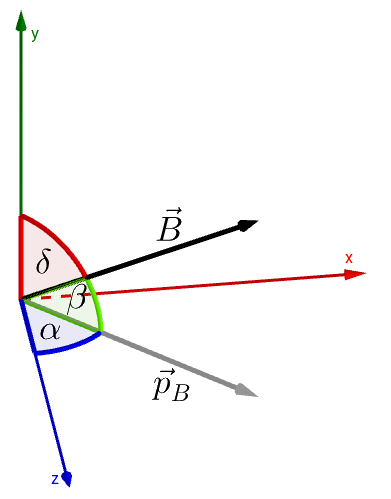
\includegraphics[width=0.45\textwidth]{geogebra/img/winkel_edited}
  \caption{Illustration der Winkel \(\alpha\), \(\beta\) und \(\delta\), die zur Drehung der \(z\)-Achse ben\"otigt werden.}
  \label{fig:winkelfig}
\end{figure}

\noindent{}Der Winkel \(\alpha\) l\"asst sich bestimmen, indem \(\vec{B}\) zun\"achst orthogonal auf die \(xz\)-Ebene projiziert wird. \(\alpha\)
entspricht dann genau dem Winkel zwischen dem aus der Projektion resultierenden Vektor \(\vec{p}_B\) und \(\vec{z}\).
Um \(\vec{B}\) auf die \(xz\)-Ebene zu projizieren, kann einfach \(\vec{B}_y=0\) gesetzt werden. Zur Berechnung des Winkels
zwischen \(\vec{p}_B\) und \(\vec{z}\)
wird folgender Zusammenhang verwendet, der f\"ur den Winkel zwischen zwei beliebigen Vektoren \(\vec{a}\) und \(\vec{b}\) gilt:
\begin{equation}
  \sphericalangle{\left(\vec{a},\vec{b}\right)} = \arccos{\left(\frac{\vec{a} \cdot \vec{b}}{\norm{a}_2 \cdot \norm{b}_2}\right)}
\end{equation}
wobei \(\norm{\cdot}_2\) der euklidischen Norm entspricht. Da \(\vec{z}\) Einheitsvektor ist, gilt \(\norm{\vec{z}}_2 = 1\),
weiterhin ist
\(\vec{z}_x = \vec{z}_y = 0\), weshalb \(\vec{z} \cdot \vec{p}_B = \vec{p}_{B_z} = \vec{B}_z\). Insgesamt ergibt sich also f\"ur den
Winkel \(\alpha\):
\begin{equation}
  \label{eq:alpha}
  \alpha = \arccos{\left(\frac{\vec{B}_z}{\norm{\vec{p}_B}}_2\right)}
\end{equation}
Da man durch Anwendung dieser Formel ausschlie{\ss}lich Winkel im Bereich von \(0 \leq \alpha \leq \pi\) erh\"alt, ist noch eine kleine
Anpassung n\"otig, damit auch im Falle eines \"uberstumpfen Winkels korrekt gedreht werden kann. Dieser Fall l\"asst sich erkennen,
indem die \(x\)-Koordinate von \(\vec{p}_B\) \"uberpr\"uft wird. Ist diese positiv, sind keine weiteren Anpassungen notwendig,
ist sie negativ, kann einfach in die andere Richtung, also um den Winkel \(-\alpha\) gedreht werden, es ergibt sich also:
\begin{equation}
  \alpha = -\arccos{\left(\frac{\vec{B}_z}{\norm{\vec{p}_B}}_2\right)}
\end{equation}
F\"ur den Fall, dass \(\vec{p}_B\)
gerade dem Nullvektor entspricht, also dass \(\vec{B}\) genau in Richtung der \(y\)-Achse zeigt, entf\"allt die Notwendigkeit
der Drehung. Hier kann formal \(\alpha = 0\) gesetzt werden.

Um nun den Drehwinkel \(\beta\) zu bestimmen, der die Drehung um die \textit{lokale} mitgedrehte \(x\)-Achse beschreibt, wird
zun\"achst der Winkel \(\delta\) berechnet, welcher den Winkel zwischen der \(y\)-Achse, im Folgenden mit \(\vec{y}\) bezeichnet,
und \(\vec{B}\) angibt. Der Winkel \(\beta\) ergibt sich dann anschaulich aus dem Zusammenhang
\(\beta = -\left(\frac{\pi}{2} - \delta\right) = \delta - \frac{\pi}{2}\). Das \(-\) r\"uhrt daher, dass in diesem Fall entgegen
der mathematisch positiven Drehrichtung gedreht wird. Auch hier muss der Fall \(\vec{B}_y < 0 \) um der Drehrichtung willen
gesondert betrachtet werden: Da hier genau entgegengesetzt gedreht werden muss, entf\"allt das \(-\) und es gilt
\(\beta = \frac{\pi}{2} - \delta\). Zeigt die gedrehte \(z\)-Achse analog zum vorigen Fall bereits in
Richtung \(\vec{B}\), so entf\"allt auch
hier die Notwendigkeit der Drehung, und es kann \(\beta = 0\) gesetzt werden. Analog zu den obigen \"Uberlegungen berechnet sich
\(\delta\) f\"ur \(\vec{B}_y \geq 0\) zu
\begin{equation}
  \delta = \arccos{\left(\frac{\vec{B}_y}{\norm{\vec{B}}}_2\right)}
\end{equation}
und f\"ur \(\vec{B}_y < 0 \) zu
\begin{equation}
  \delta = \arccos{\left(\frac{-\vec{B}_y}{\norm{\vec{B}}}_2\right)}
\end{equation}
Da die \(z\)-Achse nun durch diese beiden Drehungen erfolgreich auf \(\vec{B}\) gedreht wurde, fehlt im n\"achsten Schritt nur noch
die Drehung von \(\vec{v}\), so dass die orthogonale Projektion von \(\vec{v}\) auf die \(xy\)-Ebene genau auf der \(y\)-Achse
liegt. Der Winkel \(\gamma\), welcher zu diesem Zweck ben\"otigt wird, kann leicht ermittelt werden, indem man den Winkel zwischen
der Projektion \(\vec{p}_v\) und \(\vec{y}\) bestimmt, wie in \fref{fig:winkelv} gezeigt wird.
Analog zu den obigen Ergebnissen berechnet sich dieser f\"ur \(\vec{p}_{v_x} \geq 0\) zu
\begin{equation}
  \gamma = \arccos{\left(\frac{\vec{v}_y}{\norm{\vec{p}_v}_2}\right)}
\end{equation}
aufgrund der umgekehrten Drehrichtung im Falle von \(\vec{p}_{v_x} < 0\) ergibt sich hier
\begin{equation}
  \gamma = -\arccos{\left(\frac{\vec{v}_y}{\norm{\vec{p}_v}_2}\right)}
\end{equation}

\begin{figure}[h]
  \centering
  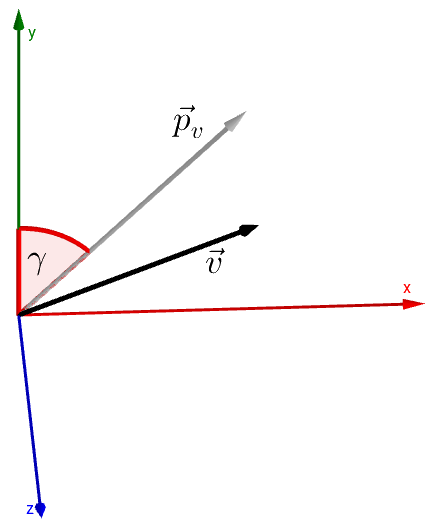
\includegraphics[width=0.45\textwidth]{geogebra/img/winkel_v_edited}
  \caption{Darstellung des Winkels \(\gamma\), welcher zur Transformation von \(\vec{v}\) ben\"otigt wird.}
  \label{fig:winkelv}
\end{figure}

\subsubsection{Zusammenfassung der Transformationsschritte}
Unter Verwendung der zuvor bestimmten Drehwinkel, kann nun die vollst\"andige Transformationsvorschrift angegeben
werden, die den \"Ubergang vom \textit{globalen} ins \textit{lokale} Bezugssystem des Ladungstr\"agers beschreibt. Im ersten Schritt
muss hierzu die Position des Teilchens in den Ursprung verschoben werden. F\"ur die relevanten Vektoren \(\vec{B}\) und \(\vec{v}\)
hat dies keine Auswirkungen, sie bleiben davon unbeeinflusst. Im n\"achsten Schritt m\"ussen die beschriebenen Drehungen
durchgef\"uhrt werden. Da sich \(\alpha\) und \(\beta\) darauf beziehen, wie die \(z\)-Achse auf \(\vec{B}\) gedreht wird, wir aber
\(\vec{B}\) auf die \(z\)-Achse drehen wollen, erhalten wir aus obigen \"Uberlegungen die \textit{inverse} der gew\"unschten
Transformation \(T_B\), die sich aus den \textit{Eulerschen Winkeln} \(\alpha\) und \(\beta\) ergibt:
\begin{equation}
  T_B^{-1} = R_y(\alpha) \cdot R_x(\beta)
\end{equation}
Nach \fref{eq:gesamtdrehung} l\"asst sich hieraus die Drehung von \(\vec{B}\) auf die \(z\)-Achse wie folgt berechnen:
\begin{equation}
  T_B = R_x(-\beta) \cdot R_y(-\alpha)
\end{equation}
Die anschlie{\ss}ende Transformation von \(\vec{v}\) ergibt sich dann zu
\begin{equation}
  T_v = R_z(\gamma)
\end{equation}
Aus diesen beiden Matrizen l\"asst sich dann die Gesamttransformation wie folgt berechnen:
\begin{equation}
  T = T_v \cdot T_B = R_z(\gamma) \cdot R_x(-\beta) \cdot R_y(-\alpha)
\end{equation}
Durch diese Matrix \(T\) l\"asst sich also jeder beliebige Vektor in das lokale Bezugssystem des Ladungstr\"agers \"uberf\"uhren.
Nachdem die in \fref{sec:lokales_bezugssystem} beschriebenen Berechnungen in dieser Basis durchgef\"uhrt wurden,
m\"ussen die Gr\"o{\ss}en dann im
Anschluss wieder in die alte Basis zur\"ucktransformiert werden. Zu diesem Zweck kann die \textit{inverse} Matrix von \(T\)
wie folgt bestimmt werden:
\begin{equation}
  T^{-1} = T_B^{-1} \cdot T_v^{-1} = R_y(\alpha) \cdot R_x(\beta) \cdot R_z(-\gamma)
\end{equation}
Die Verschiebung der Teilchenposition muss nach Anwendung der lokalen Berechnungsvorschriften ebenfalls r\"uckg\"angig gemacht werden.

\section{Ausweitung auf inhomogene Magnetfelder}

Nachdem die Flugbahnen bewegter Ladungstr\"ager in \textit{homogenen} Magnetfeldern nun ohne weiteres bestimmt werden k\"onnen, kann
das Verfahren im n\"achsten Schritt auf \textit{inhomogene} Magnetfelder ausgeweitet werden. Zu diesem Zweck wird das Verfahren
auf mehrere Iterationen heruntergebrochen. In jedem Iterationsschritt wird das magnetische Feld in der lokalen Umgebung des Teilchens
durch ein \textit{homogenes} Magnetfeld approximiert. In dieser Approximation wird anschlie{\ss}end die neue Position des
Ladungstr\"agers bestimmt, ausgehend von dieser neuen Position kann dann wieder ein lokales homogenes Magnetfeld zur N\"aherung
verwendet werden. Im Rahmen dieser Vorgehensweise wird also eine Diskretisierung des inhomogenen Feldes vorgenommen. Das inhomogene
Feld wird dabei in lokal homogene Teilfelder zerteilt, auf denen die bekannten Berechnungsvorschriften zur Anwendung kommen.

\subsection{Diskretisierung inhomogener Magnetfelder}

Um nun inhomogene Magnetfelder diskretisieren zu k\"onnen, muss im ersten Schritt die lokale Feldst\"arke \(\vec{B}\) an der Position
des Teilchens bestimmt werden. Aufbauend auf \(\vec{B}\) und der Teilchengeschwindigkeit \(\vec{v}\) k\"onnen anschlie{\ss}end nach
der notwendigen Transformation die Berechnungsvorschriften aus dem lokalen Bezugssystem angewendet werden. Zur Diskretisierung stellt
sich nun noch die
Frage, wie fein bzw. grob das inhomogene Feld unterteilt werden soll. Diese Unterteilung l\"asst sich leicht \"uber die
Simulationszeit \(t\) steuern. Beschr\"ankt man die Simulation der Flugbahn unter
Verwendung des lokalen homogenen Modells nur auf einen kurzen Zeitabschnitt \(t\), so ist die Unterteilung fein. Erh\"oht man \(t\),
so erh\"alt man eine gr\"obere Diskretisierung. Die Zeit \(t\) wird also zum Diskretisierungsparameter des Verfahrens. Je kleiner
die einzelnen Zeitabschnitte sind, in die die Gesamtsimulation unterteilt wird, desto feiner wird diskretisiert und desto geringer
sind die Abweichungen von den tats\"achlichen Gr\"o{\ss}en.

\section{Abbruchkriterien}

Nachdem beschrieben wurde, welche einzelnen Schritte in jeder Iteration durchzuf\"uhren sind, muss nun noch entschieden werden,
wann die Iteration abgebrochen werden soll. Abh\"angig vom tats\"achlichen Einsatzgebiet des Verfahrens sind hierzu verschiedene
Abbruchkriterien denkbar.
Die hier aufgelisteten m\"oglichen Bedingungen zur Beendigung der Iteration werden im Folgenden kurz erl\"autert.
\begin{itemize}
\item Schnittpunkt der Flugbahn mit einer Ebene
\item Zur\"ucklegen einer maximalen Distanz
\item Wechsel der Detektorgeometrie
\item Passieren eines bestimmten Ortes
\end{itemize}

\paragraph{Schnittpunkt der Flugbahn mit einer Ebene}
Oft k\"onnen bestimmte r\"aumliche Bereiche, in denen die Simulation der Teilchenflugbahn nicht weiter gew\"unscht ist, durch
Ebenen abgetrennt werden. Durchquert das Teilchen auf seinem Weg eine solche Ebene, die den \"Ubergang in einen derartigen Bereich
markiert, so kann die Simulation abgebrochen werden.

\paragraph{Zur\"ucklegen einer maximalen Distanz}
M\"ochte man die Ausdehnung der Flugbahn \"uber die zur\"uckgelegte Distanz beschr\"anken, so kann dieses Kriterium zur Anwendung
kommen. Unter Verwendung eines Bezugspunktes kann in jedem Iterationsschritt die aktuelle Distanz zu diesem Punkt berechnet werden,
\"uberschreitet diese eine gegebene Schwelle, f\"uhrt dies gem\"a{\ss} der Bedingung zum Abbruch der Iteration.

\paragraph{Wechsel der Detektorgeometrie}
Liegen Informationen \"uber den Aufbau des verwendeten Teilchendetektors vor, kann mithilfe dieser Bedingung der \"Ubergang in
irrelevante Bereiche des Detektors erfragt werden. Gelangt das Teilchen auf seinem Weg in solche Detektorabschnitte, so kann die
Simulation beendet werden.

\paragraph{Passieren eines bestimmten Ortes}
Unter Umst\"anden ist die Flugbahn des Teilchens nur solange von Interesse, bis dieses einen bestimmten Ort passiert hat. Hier
kann in jedem Iterationsschritt der aktuelle Abstand zwischen der Teilchenposition und dem gegebenen Ort berechnet werden.
Erreicht diese Distanz in einem Schritt ihr Minimum und w\"achst im n\"achsten Iterationsschritt wieder an, so wird die
Simulation abgebrochen.
\\
\\
Je nach Anwendungsfall ist es also unterschiedlich, welche der Bedingungen sinnvollerweise eingesetzt werden. Nat\"urlich sind
auch diverse Kombinationen und Verkn\"upfungen der verschiedenen Abbruchkriterien denkbar. Beispielsweise k\"onnte man in einem
speziellen Fall die Simulation beenden wollen, wenn das Teilchen entweder eine bestimmte Ebene schneidet, die beispielsweise eine
Seitenwand des Detektors markiert, oder wenn es eine maximale Distanz zur\"ucklegt.

Wichtig ist es, an dieser Stelle zu betonen, dass die aufgef\"uhrte Liste bei Weitem keinen Anspruch auf Vollst\"andigkeit erhebt,
das Verfahren l\"asst sich in dieser Hinsicht also beliebig erweitern und konfigurieren.

\section{Der resultierende Algorithmus}

Um abschlie{\ss}end alle Schritte zusammenzufassen, welche das Verfahren beschreiben, wird der resultierende Algorithmus im Folgenden
in Pseudocode dargestellt. Das erzielte Ergebnis der Simulation, also die Flugbahn des Ladungstr\"agers, wird hierbei durch eine
Aneinanderreihung von Teilchenzust\"anden, repr\"asentiert, die sich jeweils auf einen konkreten Zeitpunkt beziehen. Diese
Informationen werden in der Variable \textit{track} abgelegt.
\clearpage

\paragraph{Der Algorithmus in Pseudocode}
\label{sec:algorithmus}
\begin{algorithmic}[1]
  \STATE \COMMENT{Initialize variables}
  \STATE track, timeStep, particleState
  \STATE track.add(particleState)
  \WHILE{!stoppingCondition}
  \STATE \COMMENT{Get quantities}
  \STATE magneticField $\leftarrow$ getMagneticField(particleState.location)
  \STATE velocity $\leftarrow$ particleState.velocity
  \STATE oldLocation $\leftarrow$ particleState.location
  \STATE
  \STATE \COMMENT{Get angles for transformation}
  \STATE $\alpha \leftarrow$ getAlpha()
  \STATE $\beta \leftarrow$ getBeta()
  \STATE $\gamma \leftarrow$ getGamma()
  \STATE
  \STATE \COMMENT{Do the transformation}
  \STATE magneticField.rotateXY($-\beta$, $-\alpha$)
  \STATE velocity.rotateXY($-\beta$, $-\alpha$)
  \STATE velocity.rotateZ($\gamma$)
  \STATE newLocation $\leftarrow$ \(\left(0, 0, 0\right)\)
  \STATE
  \STATE \COMMENT{Calculate the characteristics of the local motion}
  \STATE $r \leftarrow$ calculateRadius()
  \STATE $\omega \leftarrow$ calculateAngularVelocity()
  \STATE $\varphi \leftarrow \omega \cdot$ timeStep
  \STATE
  \STATE \COMMENT{Update the position in the local coordinate system}
  \STATE newLocation.x $\leftarrow r \cdot \sin(\varphi) -r$
  \STATE newLocation.y $\leftarrow r \cdot \cos(\varphi)$
  \STATE newLocation.z $\leftarrow$ velocity.z $\cdot$ timeStep
  \STATE
  \STATE \COMMENT{Rotate the velocity as it follows the circular motion}
  \STATE velocity.rotateZ($\varphi$)
  \STATE
  \STATE \COMMENT{Transform back into the original system}
  \STATE velocity.rotateZ($-\gamma$)
  \STATE velocity.rotateYX($\alpha$, $\beta$)
  \STATE particleState.velocity $\leftarrow$ velocity
  \STATE particleState.location $\leftarrow$ oldLocation + newLocation
  \STATE
  \STATE \COMMENT{Set a timestamp for each particle state in the track}
  \STATE particleState.time $\leftarrow$ particleState.time + timeStep
  \STATE
  \STATE \COMMENT{Add the new state to the track}
  \STATE track.add(particleState)
  \ENDWHILE
  \STATE
  \STATE \textbf{return} track
\end{algorithmic}
